\documentclass[mathserif, aspectratio=169]{beamer}
%
%%%%%%%%%%%%%%%%%%%%%%%%%%%%%%%%%%%%%%%%%%%%%%%%%%%%%%%%%%%%%%%%%%%%%%%%
% need to split the includes to make spell checking work.
\usepackage{arev, arevmath}
\usepackage[scaled]{cabin}
\usepackage[T1]{fontenc}
\usepackage[super]{nth}
\usepackage{pifont}
\usepackage{wasysym}
\usepackage{tabularx}
\usepackage{array}
\usepackage{booktabs}
\usepackage{boldline}
\usepackage{colortbl}
%\usepackage{amsmath}
\usepackage{bm}
\usepackage{tcolorbox}
\usepackage{adjustbox}
\usepackage{minibox}
\usepackage{makecell}
\usepackage{adjustbox}
\usepackage{textcomp}
\usepackage[absolute,overlay]{textpos}
\setlength{\TPHorizModule}{1mm}%
\setlength{\TPVertModule}{1mm}%
\tcbuselibrary{skins}

\makeatletter
\newcommand{\antsize}{\@setfontsize{\antsize}{4pt}{4pt}}
\makeatother
\newcommand{\at}{\makeatletter @\makeatother}

\newcommand{\cmark}{\ding{51}}%
\newcommand{\bottomline}[1]{\vskip0pt plus 1fill{\alert{#1}\phantom{g}\vskip 1.0mm}}

\newcommand{\Quote}[2]{%
	\begin{center} 
		\begin{minipage}{0.7\textwidth} 
			\hrule
			\vskip 3mm
			\emph{{\color{ICTPblue} ``#1''}
			
			~~~~ {\color{ICTPorange} --- #2}}
			\vskip 3mm
			\hrule
			\vskip 2mm
		\end{minipage}
	\end{center}}


\mode<presentation>%
{
	\usetheme{default}
	%\usetheme[width=2.5cm]{PaloAlto}
	\usecolortheme{dove}
	\useoutertheme{infolines}
	% oder auch nicht

	% ICTP Colors
	\definecolor{ICTPblue}{RGB}{37,86,162} % 0x255682
	\definecolor{ICTPorange}{RGB}{255,130,0} % 0xff8200
	\definecolor{ICTPgreen}{RGB}{0,100,0}
	\definecolor{ICTPdark}{RGB}{80,80,80} % 0x505050
	\definecolor{ICTPlight}{RGB}{120,120,120}
	\definecolor{ICTPbrown}{RGB}{178,91,0}

	\definecolor{codebg}{rgb}{0.95,0.95,0.95}

	% Color theme
	\setbeamercolor{alerted text}{fg=ICTPorange}
	\setbeamercolor{frametitle}{fg=ICTPblue}
	\setbeamercolor{title}{fg=ICTPblue}
	\setbeamercolor{subtitle}{fg=ICTPorange}
	\setbeamercolor{normal text}{fg=ICTPdark}
	\setbeamercolor{author in foot}{fg=ICTPblue}
	\setbeamercolor{item}{fg=ICTPblue}
	\setbeamercolor{footline}{fg=ICTPblue}
	%\setbeamercolor{item projected}{bg=ICTPorange}
	%\setbeamercolor{item projected}{fg=white}

	\setbeamertemplate{headline}
	{}
	\setbeamertemplate{frametitle}
	{
		%\textbf{{\insertframetitle\phantom{g}}}\\
		%\textbf{\insertframetitle\phantom{g}}\\
		\textbf{\underline{\insertframetitle\phantom{g}}}\\
		%\textbf{\underline{\insertframetitle}}\\
		\vskip 1.0mm
		%{\color{UOLgold}\hrule height 2pt}
		%\par
	}
	\addtobeamertemplate{frametitle}{}{\vspace{-1em}}
	\setbeamertemplate{footline}{
		{%
			\textbf{ \hskip 3.0mm\insertshorttitle\phantom{.}---\phantom{.}\insertshortinstitute\hfill\insertframenumber\,/\,\inserttotalframenumber\hskip 3.0mm} 
		}
	}

	\setbeamertemplate{navigation symbols}{}%remove navigation symbols
	\setbeamertemplate{itemize items}[circle]
	\setbeamertemplate{enumerate items}[fg=ICTPblue]
	\setbeamercolor{itemize items}{fg=ICTPblue}
	\setbeamercolor{sidebar}{bg=ICTPblue}
	\setbeamercolor{title in sidebar}{fg=ICTPorange}
	\setbeamercolor{author in sidebar}{fg=ICTPorange}
	\setbeamercolor{section in sidebar}{fg=ICTPorange}
}

%\input{tikz/common-styles}

\usepackage{graphicx}
\usepackage[latin1]{inputenc}

\graphicspath{{../figs/}{../figs/common/}{../figs/islr/}}

\title[Statistical Learning] % (optional, nur bei langen Titeln n�tig)
{\textbf{Introduction to Statistical Learning\\ {\it with applications in Python}}\\%
		\href{www.statlearning.com}%
		{\tiny\it Based on ``Introduction to Statistical Learning, with applications in R'' by Gareth James, Daniela Witten, Trevor Hastie, Robert Tibishirani}\vspace{2em}}
		\vspace{-2.5cm}{}


		\author{\href{mailto:?to=Kurt Rinnert <kurt.rinnert@cern.ch>&subject=PWF Statistical Learning}{Kurt Rinnert}}

\institute[{\href{https://www.ictp.it/physics-without-frontiers.aspx}{Physics Without Frontiers} --- \href{https://www.ictp.it/}{ICTP}}] % (optional)
{\color{ICTPblue}\bfseries \href{https://www.ictp.it/physics-without-frontiers.aspx}{Physics Without Frontiers}\\\vspace{1mm}%
\href{https://www.ictp.it/}{
\includegraphics[width=0.20\textwidth]{common/ICTP-logo-full-trans.png}}\\%
\href{https://www.liverpool.ac.uk/physics/}{
\includegraphics[width=0.2\textwidth]{common/uol_logo.png}}}

\date{}

\titlegraphic{
	\texorpdfstring{\vspace{-2.8cm}}{}
	 \begin{minipage}[b][1.3cm][b]{0.26\textwidth}\color{ICTPlight}\antsize
		Copyright \textcopyright~2019\\
		\href{mailto:?to=Kurt Rinnert <kurt.rinnert@cern.ch>&subject=PWF Statistical Learning}{Kurt Rinnert <kurt.rinnert{\tt @}cern.ch>},
		\href{mailto:?to=Kate Shaw <kshaw@ictp.it>&subject=PWF Statistical Learning}{Kate Shaw <kshaw{\tt @}ictp.it>}\\
		Copying and distribution of this file, with or without modification,
		are permitted in any medium without royalty provided the copyright
		notice and this notice are preserved.  This file is offered as-is,
		without any warranty.


		Some of the figures in this presentation are taken from ``An Introduction to
		Statistical Learning, with applications in R''  (Springer, 2013) with
		permission from the authors: G. James, D. Witten,  T. Hastie and R. Tibshirani 
	 \end{minipage}\hspace{10cm}
}


\addtocounter{framenumber}{-1}

% nicer table row separation
\renewcommand{\arraystretch}{1.2}

% color boxes
\newcommand{\tabboxset}{\tcbset{enhanced, nobeforeafter, boxrule=0pt, boxsep=0pt, colback=codebg, colframe=codebg, coltext=ICTPdark, rounded corners, arc=4pt, fonttitle={\bfseries\tiny}}}
\newcommand{\codeboxset}{\tcbset{enhanced, nobeforeafter, boxrule=0pt, boxsep=0pt, colback=codebg, colframe=codebg, coltext=ICTPdark, rounded corners, arc=4pt, fonttitle={\bfseries\tiny}}}

\newcommand{\orange}{\color{ICTPorange}}
\newcommand{\blue}{\color{ICTPblue}}
\newcommand{\dark}{\color{ICTPdark}}
\newcommand{\R}{\mathbb{R}}
\newcommand{\dat}[1]{{\footnotesize\tt\orange #1}}
\newcommand{\e}[1]{\emph{#1}}
\newcommand{\bh}{\hat{\beta}}
\newcommand{\h}{\hat}

\makeatletter
\newcommand{\includegraphicsdpi}[3]{%
	\pdfimageresolution=#1%
	\includegraphics[#2]{#3}%
	\pdfimageresolution=72%
}

\newenvironment{blurb}%
	{\begin{center}\begin{minipage}{0.6\textwidth}\footnotesize}
	{\end{minipage}\end{center}}

\newenvironment{cpage}%
	{\begin{center}\begin{minipage}{0.75\textwidth}}
	{\end{minipage}\end{center}}

\newenvironment{popblock}[2]%
	{\begin{center}\begin{minipage}{#1}\footnotesize
		\begin{tcolorbox}[colframe=codebg, colback=white, colupper=ICTPdark, title={\normalsize\bfseries\blue #2}]}
	{\end{tcolorbox}\end{minipage}\end{center}}
\makeatother

\subtitle{\bfseries%
  {Statistical Learning}\\%
  {\tiny\it what is it?, models, regression, classification, prediction, inference, accuracy, bias, variance}\\%
}
\begin{document}
\frame[plain]{
	\vskip 1.0mm
	\titlepage
	\vskip 1.0mm
}


\begin{frame}{Abstract}
	%\Quote{If you fail to prepare you are preparing to fail.}{Anonymous}

	\begin{blurb}
		We give a number of examples illustrating what statistical learning
		is about.
		
		The emphasis not on particular methods but on the foundational concepts.

	\end{blurb}
\end{frame}

\begin{frame}{Overview}
	\begin{itemize}
		\item Models
		\item Prediction \& inference
		\item Accuracy  \& interpretability
		\item Bias \& Variance
		\item Regression \& classification
	\end{itemize}
	\bottomline{This sets the stage for the remainder of the course.}
\end{frame}

\begin{frame}{Example: Advertising}
	\begin{itemize}
		\item We are hired to increase the sales of a particular product.
		\item We are given the \dat{Advertising} data set.
			\begin{itemize}
				\item \dat{sales} for 200 different markets.
				\item advertising budgets for \dat{TV}, \dat{radio} and \dat{newspaper}.
			\end{itemize}
		\item Our clients can \emph{not directly} influence the sales.
		\item But they \emph{can} control the advertising budgets.
		\item We need to determine whether there is an association \\
			between advertising and sales. 
	\end{itemize}
	\bottomline{This is a typical scenario.}
\end{frame}

\begin{frame}[t]{Example: Advertising}
	\vspace{-5mm}
	\begin{center}
		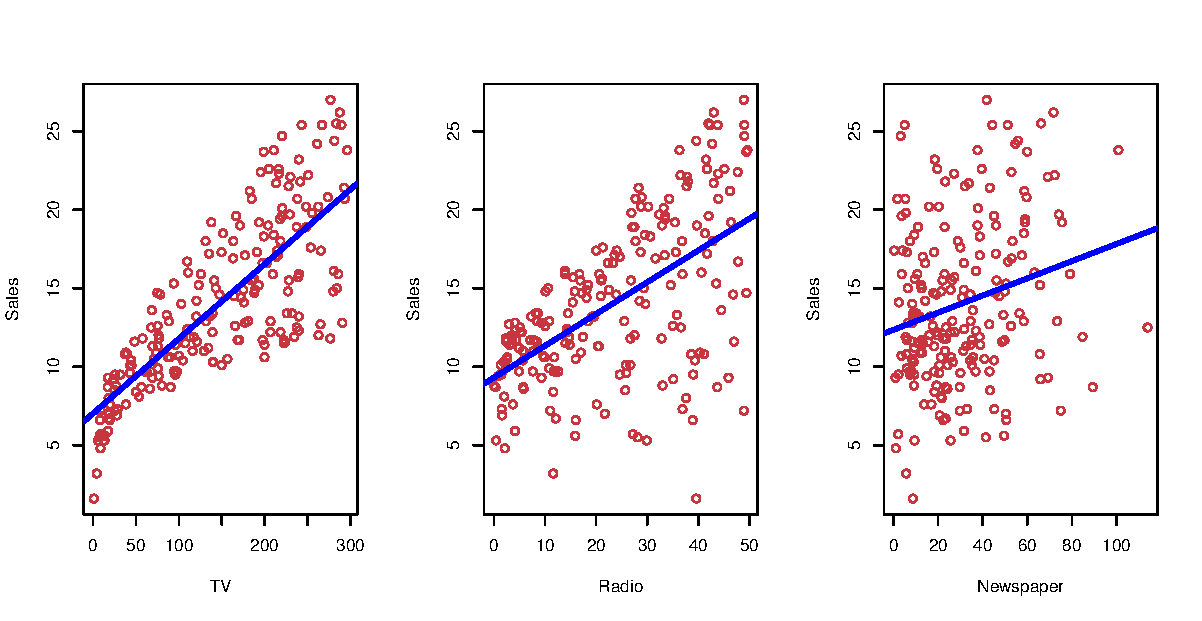
\includegraphics[width=0.6\textwidth]{2_1}
	\end{center}
	\vspace{-5mm}
	\begin{itemize}
		\item The plots display \dat{sales} as a function of the advertising budgets.
		\item Each plot is a \emph{scatter plot} of \dat{sales} versus a budget.
		\item We have overlaid a \emph{least squares line} fit on each plot.
	\end{itemize}
	\bottomline{We can already spot some promising relationships.}
\end{frame}

\begin{frame}{Example: Advertising}
	\begin{itemize}
		\item The advertising budgets are \e{input variables}.
		\item We denote the input variables with $X$.
		\item We use subscripts to distinguish them.
		\item For example, $X_1$ = \dat{TV}, $X_2$ = \dat{radio}, $X_3$ = \dat{newspaper}.
		\item The input variables are also called \e{predictors}, \e{independent variables}, \\
			\e{features} or simply \e{variables}.
		\item \dat{sales} is the \e{output variable}.
		\item Output variables are also called \e{dependent variables} or \e{responses}.
		\item We denote the output variables with $Y$.
	\end{itemize}
	\bottomline{Don't get confused by different names.}
\end{frame}

\begin{frame}{Models}
	\begin{itemize}
		\item Suppose we observe a \e{quantitative} response $Y$,\\
			and $p$ different predictors, $X_1, X_2, \dots X_p$. 
		\item We assume that there is some relationship between $Y$ and $X$.
		\item We can write this in the very general form
			\[ Y = f(X) + \epsilon\]
		\item Here $f$ is a fixed but unknown function of $X = (X_1, X_2, \dots, X_p)$.
		\item And $\epsilon$ is a random error term, independent of $X$ with mean zero.
		\item We say $f$ represents the \e{systematic} information\\
			that $X$ provides about $Y$.
	\end{itemize}
	\bottomline{This is the most general form of a \e{model}.}
\end{frame}

\begin{frame}{Example: Income}
	\vspace{-5mm}
	\begin{center}
		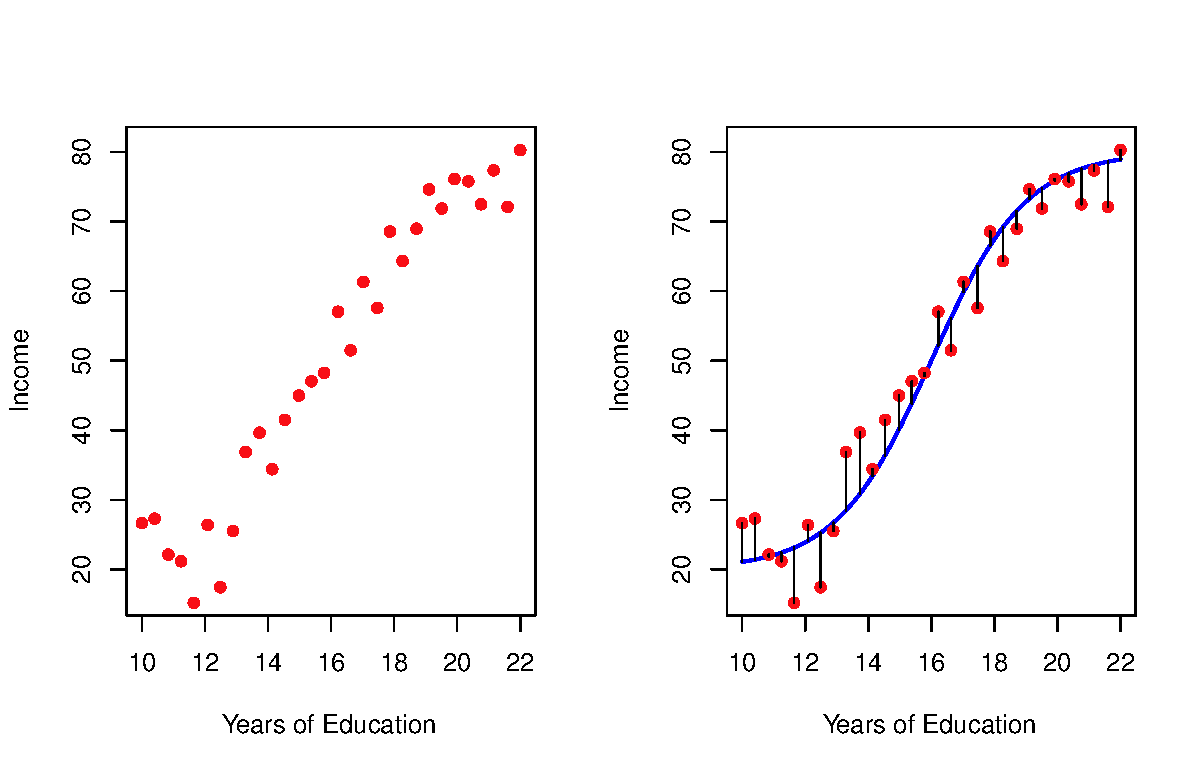
\includegraphics[width=0.5\textwidth]{2_2}
	\end{center}
	\vspace{-5mm}
	\begin{itemize}
		\item The figure shows a scatter plot of \dat{income} versus \dat{years of education}.
		\item The blue curve is the true functional relationship $f(X) =f(X_1)$.
		\item The vertical lines represent the error terms $\epsilon$.
	\end{itemize}
	\bottomline{This is a simulated data set.}
\end{frame}

\begin{frame}{Example: Income}
	\vspace{-5mm}
	\begin{center}
		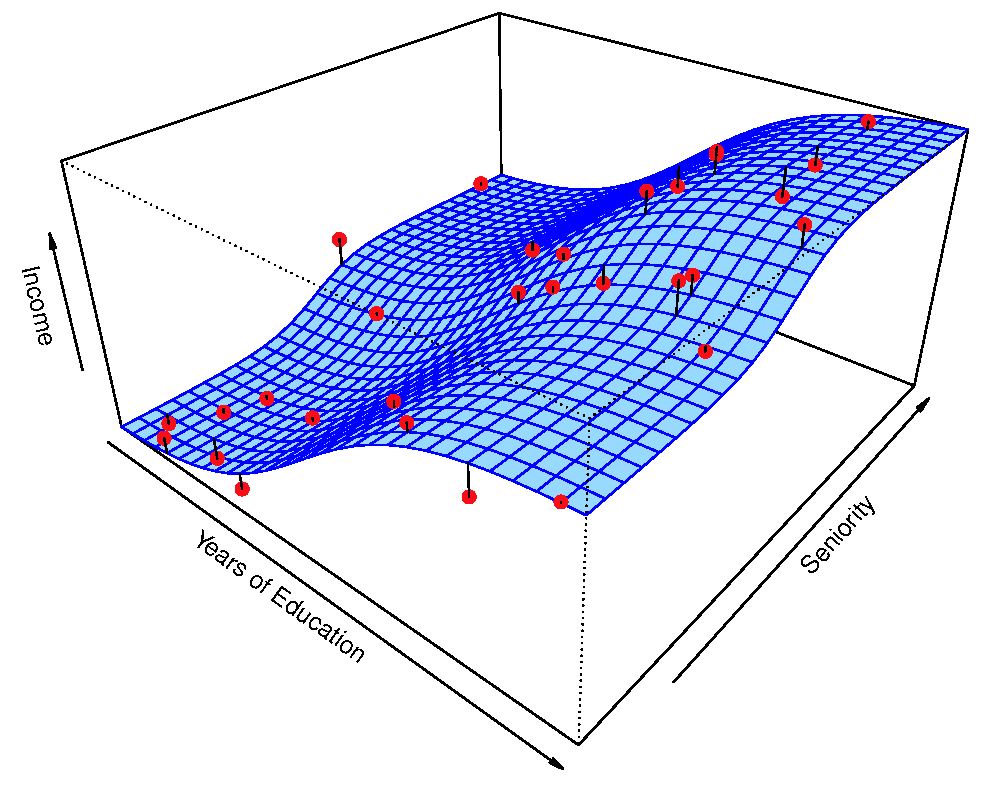
\includegraphics[width=0.4\textwidth]{2_3}
	\end{center}
	\vspace{-5mm}
	\begin{itemize}
		\item The figure shows a 3D scatter plot of \dat{income} versus \dat{years of education}
			and \dat{seniority}.
		\item The blue surface is the true functional relationship $f(X) = f(X_1, X_2)$.
		\item The vertical lines represent the error terms $\epsilon$.
	\end{itemize}
	\bottomline{Visualising higher dimensions is hard.}
\end{frame}

\begin{frame}{What is Statistical Learning?}
	\begin{blurb}
		In essence, statistical learning refers to to a set of approaches for estimating
		the function $f$.

		In this lecture we cover the key theoretical concepts that arise in estimating $f$, as well
		as techniques for evaluating the estimates obtained.
	\end{blurb}
	\bottomline{This equally applies to machine learning.}
\end{frame}

\begin{frame}{Why estimate $\bm{f}$?}
	%\begin{itemize}
		%\item There are two main reasons why we wish to estimate $f$.
	%\end{itemize}
		There are two main reasons why we wish to estimate $f$.
	\begin{enumerate}
		\item \e{Prediction}: assuming the inputs $X$ are readily available, we simply want ot
			predict
			\[\hat{Y} = \hat{f}(X)\]
			without being interested in the exact form of $\hat{f}$.
		\item \e{Inference}: we want to understand the functional relationship
			\[Y = Y(X_1, X_2, \dots, X_p)\]
			between the predictors and the response.
	\end{enumerate}
	\bottomline{We discuss each in more detail.}
\end{frame}

\begin{frame}{Prediction}
	\begin{itemize}
		\item Often the inputs $X$ are readily available but the response $Y$ is not.
		\item Since the error term $\epsilon$ averages to zero, we can then predict
			\[\hat{Y} = \hat{f}(X)\]
			where $\hat{f}$ represents the estimate of $f$ and $\hat{Y}$ is the resulting
			prediction of $Y$.
		\item In this scenario we are not interested in the exact form of $\hat{f}$.
		\item We are mostly concerned with the accuracy of $\hat{Y}$.
	\end{itemize}
	\bottomline{Here $\bm{\hat{f}}$ is often treated as a \e{black box}. But we don't have to!}
\end{frame}

\begin{frame}{Prediction Accuracy}
	\begin{itemize}
		\item The accuracy of $\hat{Y}$ depends on two quantities:
			\begin{enumerate}
				\item the \e{reducible error}
				\item the \e{irreducible error}
			\end{enumerate}
		\item The reducible error is due to $\hat{f}$ not being a perfect estimate of $f$.\\
			(We can potentially come up with better statistical learning techniques to 
			improve $\hat{f}$).
		\item Even if our estimate of the relationship was perfect ($\hat{f} = f$),\\
			our estimate $\hat{Y}$ would still have an error!
		\item This irreducible error is due to our \e{observations} not being perfect.\\
			(The error term $\epsilon$).
	\end{itemize}
	\bottomline{You have to understand what you can improve and what you can't.}
\end{frame}

\begin{frame}{Prediction Accuracy}
	\begin{itemize}
		\item Assuming that $\hat{f}$ and $X$ are fixed, we can show that
			\begin{align*}
				E[(Y - \hat{Y})^2] &= E[(f(X) + \epsilon - \hat{f}(X))^2]\\ 
				&= \underbrace{E[(f(X) - \hat{f}(X))^2]}_\text{Reducible}
				+ \underbrace{\text{Var}(\epsilon)}_\text{Irreducible} \\ 
			\end{align*}
			where $E[(Y - \hat{Y})^2]$ is the average, or \e{expected value}, of the squared\\
			difference between the predicted and the true value of $Y$,\\
			and $\text{Var}(\epsilon)$ is the \e{variance} of the error term $\epsilon$.
		\item The average $E[z]$ is often written as $\overline{z}$ or $\langle z \rangle$.
		\item The variance is then $\text{Var}(z) = \langle (z - \overline{z})^2 \rangle
			= \langle z^2 \rangle - {\langle z \rangle}^2 = \overline{z^2} - \overline{z}^2$.
	\end{itemize}
	\bottomline{All techniques we learn aim to estimate $f$ while minimising the reducible error.}
\end{frame}

\begin{frame}{Inference}
	\begin{itemize}
		\item We are often interested in \e{how} $X_1, X_2, \dots, X_p$ affect $Y$.
		\item We want to estimate $f$, but not necessarily predict $Y$.
		\item The aim is to understand the \e{functional relationship} between $Y$ and $X$.
	\end{itemize}
	\bottomline{We can \e{not} treat $\hat{f}$ as a black box in this scenario.}
\end{frame}

\begin{frame}{Inference: Questions}
	\begin{cpage}
		\begin{itemize}
			\item \e{\orange Which predictors are associated with the response?}\\
				We want to identify the \e{important} predictors.
			\item \e{\orange What is the relationship between the response and each predictor?}\\
				For example, predictors can have positive or negative influence\\
				on the response. Any functional relationship can occur, 
				possibly depending on the values of the other predictors.
			\item \e{\orange Can the relationship between $Y$ and each predictor be summarised as
				a linear equation?}
				It greatly simplifies things when the relationship can be captured by a linear model.
				Historically, models have been mostly chosen to be linear. However, the true relationships
				are very rarely linear.
		\end{itemize}
	\end{cpage}
	\bottomline{Linear is good, but rarely true.}
\end{frame}

\begin{frame}{How do we estimate $\bm{f}$?}
	\begin{columns}
		\begin{column}{0.7\textwidth}
			\begin{itemize}
				\item We have $n$ \e{observations} of $X$ and $Y$.
				\item In the plots on the right $n$ is 30.
				\item This is the \e{training data}.
				\item We use these observations to \e{train}, or \e{teach}, our model\\
					how to estimate $f$.
				\item The goal is to find a function $\hat{f}$ such that $Y \approx \hat{f}(X)$,
					for each observation $(Y, X)$.
			\end{itemize}
		\end{column}
		\begin{column}{0.3\textwidth}
			\begin{center}
				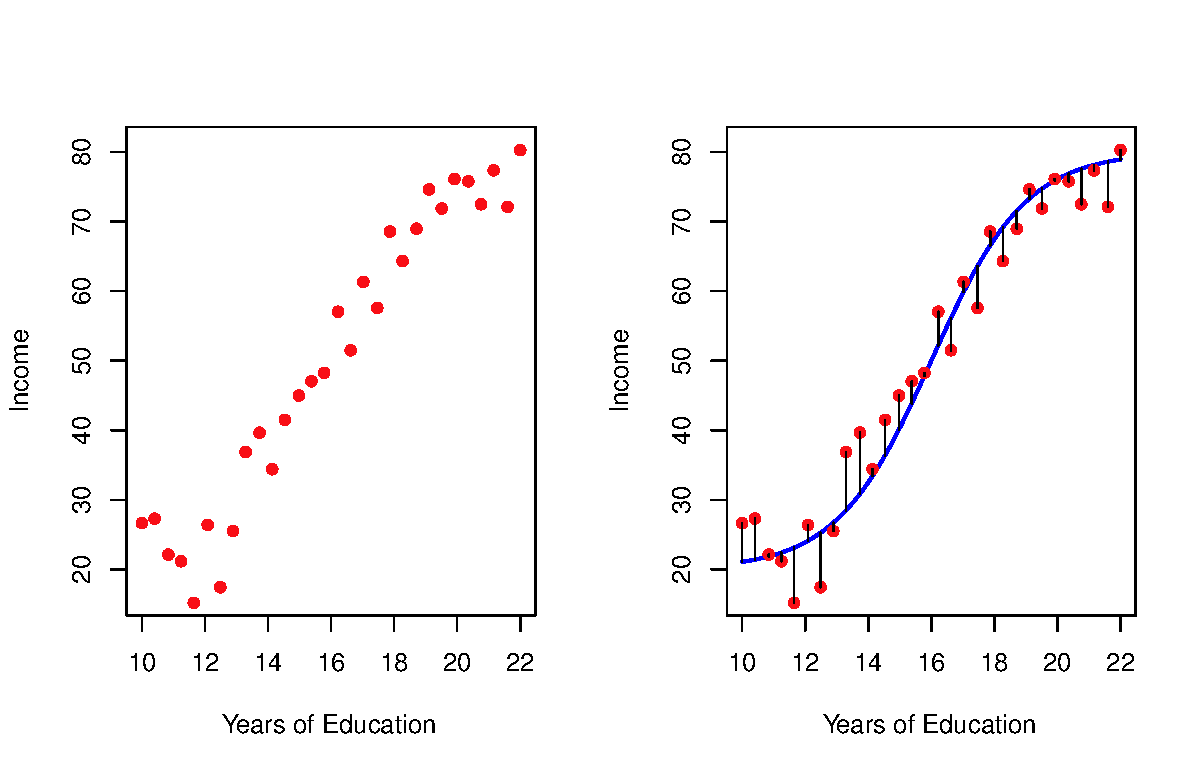
\includegraphics[width=\textwidth]{2_2}
			\end{center}
			\begin{center}
				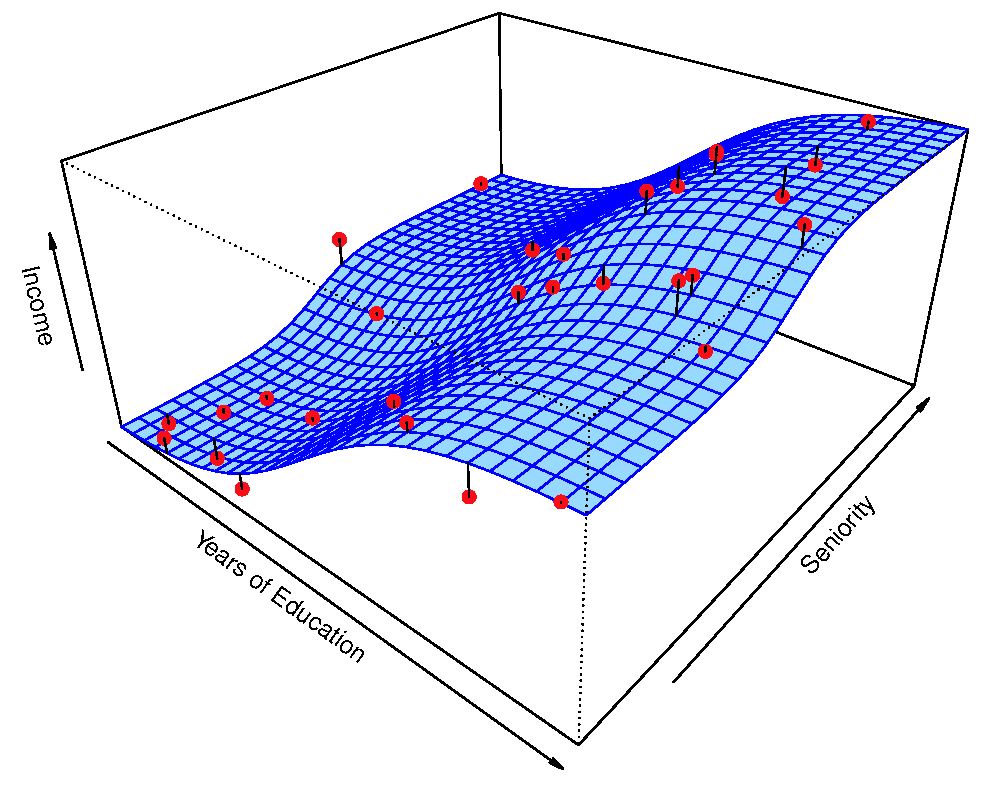
\includegraphics[width=0.9\textwidth]{2_3}
			\end{center}
		\end{column}
	\end{columns}
	\bottomline{Statistical learning methods are either \e{parametric} or \e{non-parametric}.}
\end{frame}

\begin{frame}{Parametric Methods}
	\begin{cpage}
		\begin{enumerate}
			\item \e{\orange Make an assumption about the functional form of $f$.}\\
				A very simple assumption is a linear model:
				\[ f(X) = \beta_0 + \beta_1 X_1 + \beta_2 X_2 + \dots + \beta_p X_p\]
				With a linear model we only need to estimate $p + 1$ parameters. 
				We will cover linear models in great detail in the next lecture.
			\item \e{\orange Use the training data to train, or fit, the model.}\\
				For a linear model we need to estimate the parameters 
				$\beta_0, \beta_1, \beta_2, \dots, \beta_p$ such that:
				\[ Y \approx \hat{\beta}_0 + \hat{\beta}_1 X_1 + \hat{\beta}_2 X_2 
				+ \dots + \hat{\beta}_p X_p \] 
		\end{enumerate}
	\end{cpage}
	\bottomline{Non-linear models are of course possible, but harder to fit.}
\end{frame}

\begin{frame}{Linear Model Example}
	\vspace{-5mm}
	\begin{center}
		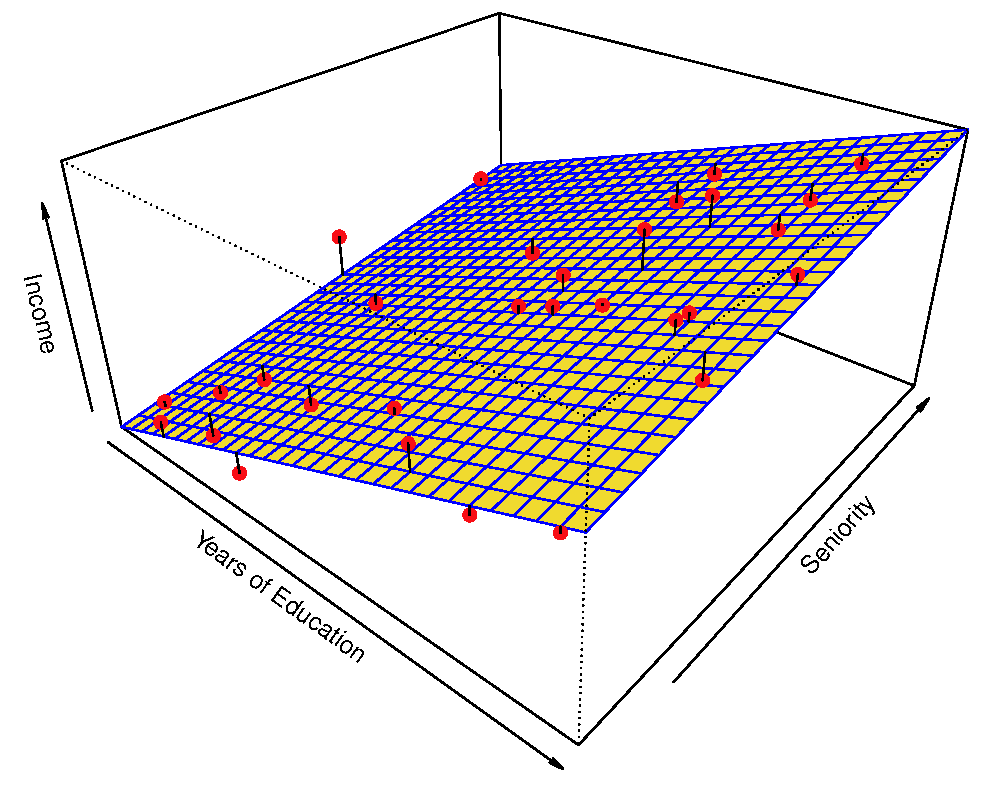
\includegraphics[width=0.5\textwidth]{2_4}

		\[ \text{\dat{income}} \approx \hat{\beta}_0 + \hat{\beta}_1\times\text{\dat{education}}
		+ \hat{\beta}_2\times\text{\dat{seniority}}\]
	\end{center}
\end{frame}

\begin{frame}{Non-parametric Methods}
	\begin{cpage}
		\begin{enumerate}
			\item \e{\orange No assumption about the functional form of $f$ is made.}\\
			\item \e{\orange Seek an estimate of $f$ that smoothly approaches the data points\\
				in the training data.}
		\end{enumerate}
		\begin{itemize}
			\item[$+$] Avoids choosing potentially very wrong models.
			\item[$+$] Can approximate any functional relationship.
			\item[$-$] Often need many more observations for the fit.
			\item[$-$] Prone to over-fitting.
		\end{itemize}
	\end{cpage}
	\bottomline{Oddly, non-parametric methods can have a lot of parameters.}
\end{frame}

\begin{frame}{Non-parametric Example}
	\vspace{-5mm}
	\begin{center}
		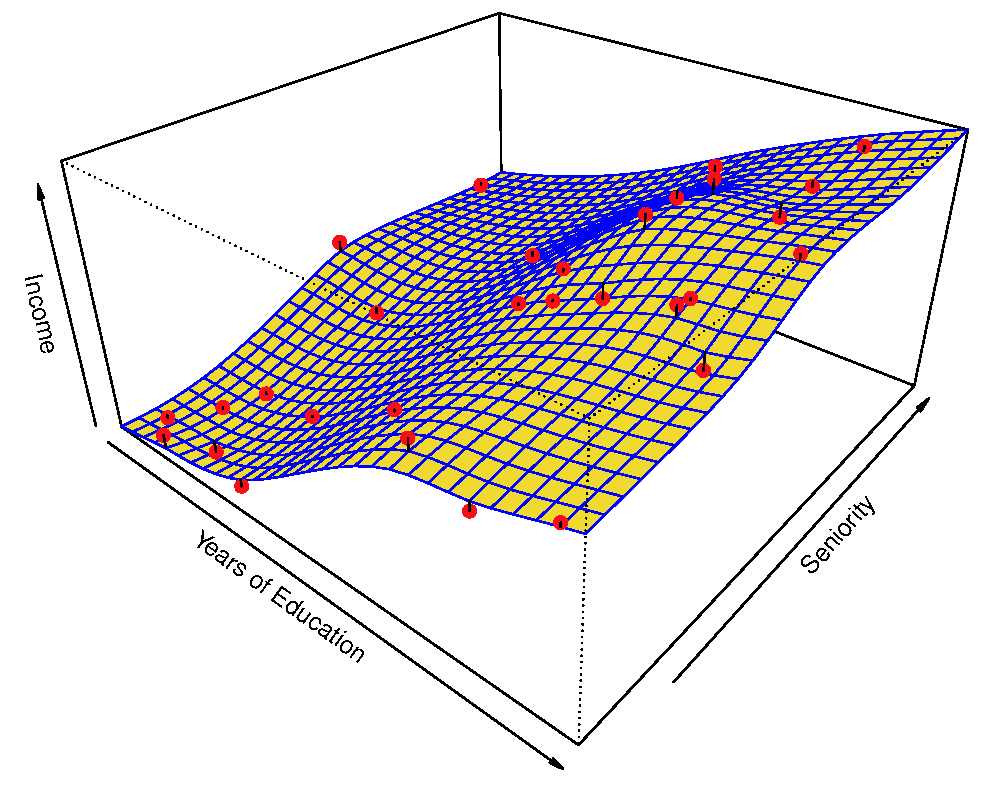
\includegraphics[width=0.5\textwidth]{2_5}

		Approximation to $f$ to predict \dat{income} using a \e{thin-plate spline}. 
	\end{center}
	\bottomline{Better fit to the training data than the linear model.}
\end{frame}

\begin{frame}{Non-parametric Example}
	\vspace{-5mm}
	\begin{center}
		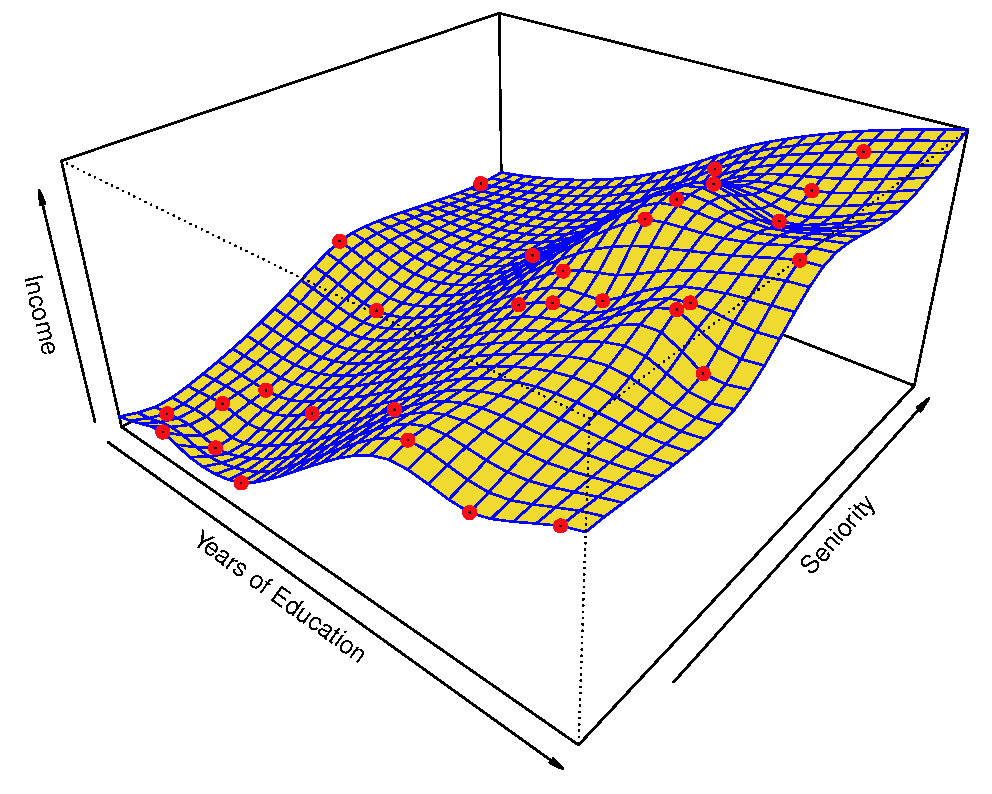
\includegraphics[width=0.5\textwidth]{2_6}

		A less smooth spline fit that fits the training data perfectly. 
	\end{center}
	\bottomline{This is an example of \e{over-fitting}.}
\end{frame}

\end{document}
